 % Formatação BR ABNT
\documentclass[
    article,
    12pt,
    oneside,
    a4paper,
    brazil,
    sumario=traditional
]{abntex2}

% Pacotes
\usepackage[letterpaper,top=2cm,bottom=2cm,left=3cm,right=3cm,marginparwidth=2cm]{geometry}
\usepackage[utf8]{inputenc}
\usepackage{csquotes}
\usepackage{listings}
%\usepackage{cite}
%\usepackage{biblatex}% pacote para citações
\usepackage{braket}% pacote para notação bracket
\usepackage{fancyhdr}% pacote para header e footer7
\usepackage{hyperref}% pacote para URLs
\usepackage{amsmath}% pacote para matrizes
\usepackage{amsfonts}
\usepackage{amssymb}
\usepackage{amsthm} % Ambientes para exemplos, teoremas, provas e definições
\usepackage{mathtools}
\usepackage{siunitx}
\usepackage{multirow}
\usepackage{booktabs}
\usepackage{array}      % Traz algumas funcionalidades úteis
\usepackage{verbatim}   % Traz algumas funcionalidades úteis
\usepackage{graphicx}   % Inclusão de figuras
\usepackage{epstopdf}   % Converte as imagens em EPS para PDF
\hypersetup{
    colorlinks=true,
    linkcolor=black,
    filecolor=magenta,
    urlcolor=black,
    citecolor=black,
    hidelinks
}
% Code and Hilighting 
\usepackage{listings}
\usepackage{xcolor}
\usepackage{dsfont}
\usepackage{pgfplots}
\usepackage{adjustbox}
%\usepackage{minted}

%Chemistry
\usepackage[version=4]{mhchem}

% \usepackage{wrapfig}
\usepackage{caption}
\usepackage{subcaption}
\usepackage{tikz} % Criação de Imagens e Gráficos
\usetikzlibrary{matrix}
\usetikzlibrary{calc}

\DeclareMathOperator{\diag}{diag}

\definecolor{codegreen}{rgb}{0,0.6,0}
\definecolor{codegray}{rgb}{0.5,0.5,0.5}
\definecolor{codepurple}{rgb}{0.58,0,0.82}
\definecolor{backcolor}{rgb}{0.95,0.95,0.92}

\lstdefinestyle{mystyle}{
    backgroundcolor=\color{backcolor},   
    commentstyle=\color{codegreen},
    keywordstyle=\color{magenta},
    numberstyle=\tiny\color{codegray},
    stringstyle=\color{codepurple},
    basicstyle=\ttfamily\footnotesize,
    breakatwhitespace=false,         
    breaklines=true,                 
    captionpos=b,                    
    keepspaces=true,                 
    numbers=left,                    
    numbersep=5pt,                  
    showspaces=false,                
    showstringspaces=false,
    showtabs=false,                  
    tabsize=2
}
\lstset{style=mystyle}
\fancyhead[R]{Otimização de Geometria Molecular}

% Configuração
% Biblatex
%\bibliographystyle{plain} % We choose the "plain" reference style
%\addbibresource{ref.bib}


\begin{document}
\thispagestyle{empty}

\begin{figure}
	\centering
	\includegraphics[scale = 0.3]{figures/logo_ufabc.eps}
	\label{fig:UFABC_logo}
\end{figure}

\begin{center}
	
	{\scshape\LARGE Universidade Federal do ABC \par}
	\vspace{1.5cm}
	{\scshape\Large Relatório Iniciação Científica \par}
	\vspace{1.5cm}
	{\huge \bfseries Otimização de Geometria Molecular \par}
	\vspace{2cm}
	{\LARGE \itshape Felipe Fernandes Gomes da Silva Costa \par}
	
	\vfill
	
	% Final da página
	{\large Santo André, SP \par}	
	{\large \today \par}
	
\end{center}

\clearpage

\thispagestyle{empty}

\begin{center}
	{\Large\itshape Felipe Fernandes Gomes da Silva Costa \par}
	\vspace{3cm}
	{\LARGE \bfseries Otimização de Geometria Molecular \par}
	\vspace{3cm}
	\begin{flushright}
		\begin{minipage}[c]{.6\textwidth}
			Relatório de Iniciação Científica.
		\end{minipage}
	\end{flushright}
		
	\vspace{3cm}
	{\scshape\Large Universidade Federal do ABC \par}
	\vfill
	{\Large Orientador: \par Prof. Dr. Yuri Alexandre Aoto}
	
	\vfill
	
	% Final da página
	{\large Santo André, SP \par}	
	{\large \today \par}
	
\end{center}


\clearpage

% header
\setlength{\headheight}{35pt}
\pagestyle{fancy}
%\begin{boldmath}
 
%\maketitle

\newpage
\tableofcontents
\newpage
%%%%%%%%%%%%%%%%%%%%%%%%%%%%%%%%%%%%%%%%%% Início %%%%%%%%%%%%%%%%%%%%%%%%%%%%%%%%%%%%%%%%%

\section{Resumo}

A otimização de geometria molecular é um tópico essencial da química
computacional, em que utilizando funções de Superfície de Energia Potencial (SEP) é possível 
predizer configurações estáveis de uma molécula ou estados de transição. 
O objetivo deste projeto foi desenvolver um algoritmo para otimização de funções SEP baseado no método
de Newton, mantendo uma taxa de convergência similar e com menor custo computacional. 
O algoritmo proposto, CBPD (Convergence Based on Partial Derivatives), foi aplicado à reação 
\ce{F + H_2O -> FH + HO}, permitindo avaliar sua eficácia em diferentes cenários de otimização. 
Comparado ao método de Newton, o CBPD mostrou boas taxas de convergência em cenários específicos,
apesar de exigir um número maior de iterações cada etapa de iteração possui um menor custo computacional.
Os resultados indicam que o CBPD pode ser uma alternativa promissora para problemas de otimização em 
química computacional de funções SEP em um espaço de alta dimensionalidade.

\clearpage

\section{Introdução}

A otimização geométrica de estruturas moleculares é um ramo de pesquisa da química
computacional que busca por meio de algoritmos identificar conformações moleculares que
são estáveis, ou que sejam uma configuração de uma etapa de uma reação química. É de interesse compreender essas conformações não apenas para o entendimento dos mecanismos das reações, mas também para aplicações práticas, como o desenvolvimento de novos fármacos.

% TODO: Reformular a ideia de que um mínimo local está associado com configurações estáveis e/ou transição, isso nem sempre é verdade, estados de transição são barreiras que dividem duas etapas da reação, uma relacionada com reagente outra com produto (são pontos estacionários instáveis).
O conceito de Superfície de Energia Potencial (SEP) (do inglês, \textit{Potential Energy Surface}) descreve que para cada configuração de uma molécula, i.e, o tamanho das ligações e ângulos em que os átomos estão arranjados, existe um valor de energia associado. Dado que uma SEP pode estar associada a uma função, localizar os pontos críticos dessa função usualmente representa identificar as configurações estáveis de uma molécula ou estados de transição, que estão diretamente relacionados com mínimos locais e pontos de sela respectivamente \cite{geometry_optimization}.

Funções que representam SEP, por conta de suas complexidades, não costumam possuir expressões analíticas. Dessa maneira, os valores de suas derivadas, que são frequentemente utilizados em métodos de otimização, passam a ser obtidos  exclusivamente por aproximações. Diante disso, é relevante que o método de otimização implementado possua uma maneira eficiente de fazer o cálculo das derivadas. 

% TODO:A afirmação (O algoritmo trata o processo de otimização de uma função multidimensional como uma soma de funções unidimensionais) não está precisa, parece que estamos dizendo algo como f(x,y) = h(x) + g(y)
O objetivo de estudo do projeto é a construção de um algoritmo baseado no Método de Newton e Método da Secante, que permita realizar a otimização de funções SEP. O algoritmo trata o processo de otimização de uma função multidimensional considerando apenas a diagonal de sua matriz hessiana, como será apresentado na seção \ref{sec:cbpd-process}. No caso, é feito a otimização de cada derivada parcial da função multidimensional utilizando o Método de Newton e aproximando os valores das derivadas parciais utilizando o Método da Secante.

Para a validação do algoritmo desenvolvido será utilizado a função SEP que descreve a reação entre fluor e água (\ce{F + H2O -> FH + HO}) \cite{fh2o_first_sep}. Apesar desta função possuir uma expressão analítica, o trabalho visa desenvolver um método genérico de convergência de funções PES. O algoritmo desenvolvido denominado CBPD (\textit{Convergence Based in Partial Derivatives}) será comparado com o Método de Newton em diferentes cenários de convergência, avaliando a taxa de convergência e a quantidade de iterações necessárias para convergir.

A organização do restante deste resumo é descrita a seguir. A Seção \ref{sec:definitions} apresenta termos fundamentais em métodos de otimização. A Seção \ref{sec:teorical-base} revisa os métodos de convergência que serão utilizados como base, assim como descreve sobre a reação de estudo. A metodologia utilizada nesse projeto é descrita na Seção \ref{sec:methodology}. Por fim os resultados e conclusões são apresentados nas Seções \ref{sec:results} e \ref{sec:conclusions} respectivamente.

\clearpage

\section{Definições}
\label{sec:definitions}

\subsection{Otimização}

O processo de otimização do contexto desse trabalho consiste em localizar os mínimos locais da função que descreve a superfície de energia potencial que está sendo estudada. Nesse processo, fornecendo uma geometria inicial da molécula em estudo, ou seja, um valor inicial para os argumentos da função que descreve a SEP, será retornado a geometria em que a SEP tem valor mínimo local. O processo é feito por iterações até que o algoritmo de otimização consiga convergir (otimizar) ou chegue no limite de iterações definidas.

\subsection{Iterações}

Uma iteração, nesse contexto, consiste em cada etapa no processo de otimização. Inicialmente temos ponto do domínio da função, é realizado então a etapa de convergência, que é justamente o enfoque do projeto, que consiste em realizar um processo matemático para definir um próximo ponto do domínio que idealmente deve ser mais próximo do mínimo local da função. Caso o novo ponto definido esteja próximo o suficiente do mínimo local, é dito que o algoritmo convergiu e o processo de otimização é finalizado. A definição se o ponto está próximo o suficiente é feita com o uso de norma, no projeto atual está sendo usado a norma euclidiana. Para cada novo ponto é calculada a norma do gradiente da função, caso esse valor seja igual ou menor a um valor de tolerância é definido que algoritmo convergiu. O valor de tolerância é um parâmetro que define o quão próximo o ponto deve estar do mínimo local para ser considerado que o ponto está no ponto mínimo. Quanto menos iterações forem feitas e quanto menor o custo computacional envolvido em cada iteração, é dito que o algoritmo é mais eficiente.

\clearpage

\section{Fundamentação Teórica}
\label{sec:teorical-base}
  O processo de otimização pode ser realizado com diferentes métodos, que nesse contexto possuem o mesmo objetivo, localizar as raízes de uma função, seja essa função fornecida analiticamente ou numericamente. Todo método existente possui seus pontos positivos e negativos dentre os demais, seja por sua eficiência, facilidade de implementação ou custo computacional relacionado a cada etapa da iteração. A pesquisa está se embasando principalmente sobre o Método de Newton, que satisfazendo seus critérios de convergência \cite{calculo_numerico_aplicado} é classificado como estável, ou seja, a cada iteração é obtido um novo ponto mais próximo da região de convergência que possui um erro relativo menor quando comparado com a etapa anterior.

\subsection{Método de Newton}
\label{sec:newton-method}

No Método de Newton, dado um ponto inicial, utilizando a derivada da função em estudo, se obtém um próximo ponto mais próximo da região de convergência. Nesse processo, iniciamos de um ponto inicial arbitrário da função e traçamos uma reta tangente da função no ponto, ou seja, verificamos o valor da derivada no ponto e utilizamos para definir uma função afim $g: {\mathds{R}\to\mathds{R}}$ com $g(x) = ax + b$, $a, b \in \mathds{R}$. Com a função afim definida no ponto, identificamos a raiz da função, ou seja, definimos o ponto em que $g(x)=0$.

Podemos calcular o ponto $x_n$ em que $g(x) = 0$ da seguinte maneira:
%
\begin{equation}
  x_n = x_{n-1} - \frac{f(x)}{f'(x)}
\end{equation}
%
Realizamos novamente o processo anterior, agora para o ponto $f(x_n)$. Para cada novo ponto $x_k$ obtido aproximamos cada vez mais do ponto em que $f(x_k)$ é igual a zero.


\subsection{Método da Secante}

O Método da Secante utiliza dois pontos da função para calcular o próximo ponto da iteração com o objetivo que seja mais próximo da raíz da função. Cada iteração é calculada com base na reta formada pelos dois pontos anteriores, que será secante ao gráfico da função. Dessa forma, o ponto $x_n$ é definido:
%
\begin{equation}
  x_n = x_{n-1} - f(x_{n-1}) \frac{x_{n-1} - x_{n-2}}{f(x_{n-1}) - f(x_{n-2})} \,.
\end{equation}
%
Trazendo enfoque na etapa de iteração, mais precisamente no termo relativo a reta secante
%
\begin{equation}
  \frac{x_{n-1} - x_{n-2}}{f(x_{n-1}) - f(x_{n-2})} \,,
\end{equation}
%
se definirmos $x_{n-1} = x_{n-2} + h$ com $h \in \mathds{R}$ temos
%
\begin{equation}
  \frac{x_{n-2} + h - x_{n-2}}{f(x_{n-2} + h) - f(x_{n-2})} = \frac{h}{f(x_{n-2} + h) - f(x_{n-2})} \,.
\end{equation}
%
Podemos tomar o inverso dessa expressão, e, para casos em quem que a distância dentre os dois pontos seja suficientemente pequena, ou seja, caso o valor de $h$ tenda a $0$, o termo representado passa a ser o inverso de uma aproximação da derivada no ponto.
%
\begin{equation}
  \Bigg( \frac{f(x_{n-2} + h) - f(x_{n-2})}{h} \Bigg)^{-1} \approx \Bigg( \lim\limits_{h\to0}\frac{f(x_{n-2}+h)-f(x_{n-2})}{h} \Bigg)^{-1} = \Bigg( \frac{df}{dx}(x_{n-2}) \Bigg)^{-1}
\end{equation}
%
Além disso, notemos que a função $f$ é diferenciável, o Teorema do Valor Médio\cite{calculo_1} afirma que existe uma reta tangente entre os dois pontos $x_{n-1}$ e $x_{n-2}$ que o seu valor é exatamente o valor da reta secante calculada.

\subsection{Método de Newton Multidimensional}

O Método de Newton Multidimensional consiste em uma generalização do Método de Newton porém para casos que possam envolver funções multidimensionais. Sejam uma função $F: {\mathds{R}^k\to\mathds{R}^k}$ com $k \in \mathds{N}$ e $\mathbf{x}_n \in \mathds{R}^k$ referente ao enésimo ponto do processo de otimização. Um novo ponto $\mathbf{x}_{n+1}$ é definido por:
%
\begin{equation}
  \label{eq:newton_generalization}
  \mathbf{x}_{n+1} = \mathbf{x}_n - J_F(\mathbf{x}_n)^{-1}F(\mathbf{x}_n) \,,
\end{equation}
%
sendo $J_F(\mathbf{x}_n)^{-1}$ a matriz inversa $k \times k$ do Jacobiano da função $F$.

É importante se atentar nesse método sobre quais condições a etapa de iteração pode performar. Nesse caso é sempre necessário verificar se a matriz $J_F(\mathbf{x}_n)$ é inversível, ou seja, $\det(J_F(\mathbf{x}_n)) \neq 0$, pois caso contrário não é possível dar sequência no processo de otimização.

\subsection{Reação \ce{F + H2O -> FH + HO}}

Nessa pesquisa será estudada a reação de \ce{F + H2O -> FH + HO} que passa por 5 pontos estacionários. Cada ponto estacionário possui uma conformação específica que permitem que os reagentes interajam. No caso em estudo são:
%
%\begin{itemize}[itemsep=0pt,parsep=0pt]
\begin{itemize}
  \setlength\itemsep{0pt}
  \setlength\parsep{0pt}
  \item Reagentes
  \item R-vdW
  \item TS
  \item P-vdW
  \item Produtos
\end{itemize}

% \begin{wrapfigure}{r}{0.6\textwidth}
\begin{figure}
  \begin{center}
    \pgfdeclarelayer{background}
\pgfsetlayers{background,main}

\newcommand{\Bond}[6]%
% start, end, thickness, incolor, outcolor, iterations
{ 
  \begin{pgfonlayer}{background}
    \colorlet{InColor}{#4}
    \colorlet{OutColor}{#5}
    \foreach \I in {#6,...,1}
      {
        \pgfmathsetlengthmacro{\r}{#3/#6*\I}
        \pgfmathsetmacro{\C}{sqrt(1-\r*\r/#3/#3)*100}
        \draw[InColor!\C!OutColor, line width=\r] (#1.center) -- (#2.center);
      }
  \end{pgfonlayer}
}

\newcommand{\SingleBond}[2]%
% start, end
{   
  \Bond{#1}{#2}{0.7mm}{white}{black!75}{10}
}

\begin{center}
  
  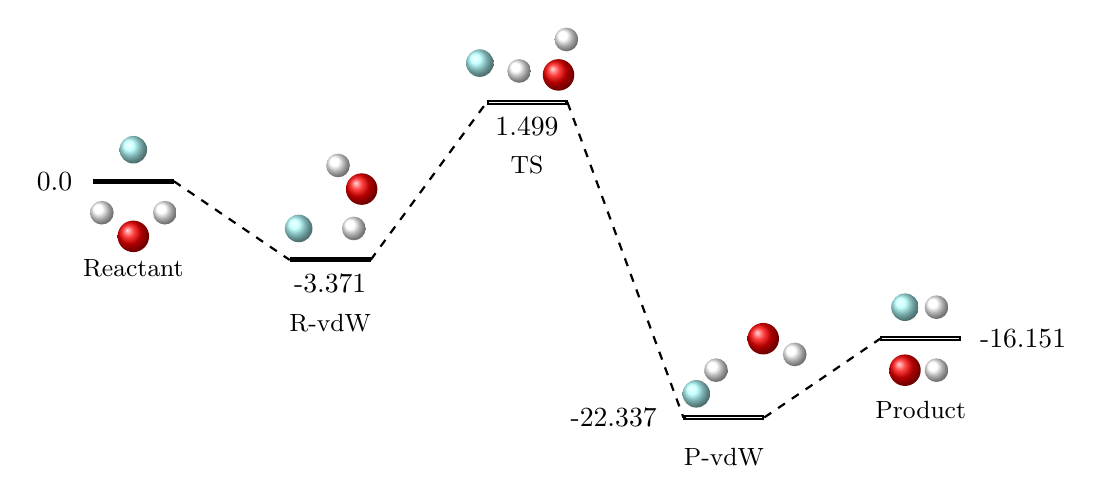
\begin{tikzpicture}[
      scale = 1,
      plateau/.style = {
        draw,
        thick,
        rectangle,
        minimum width = 1cm,
        inner sep = 0pt
      },
      oxygen/.style = {
        circle,
        ball color=red,
        minimum size=4mm,
        inner sep=0
      },
      hydrogen/.style = {
        circle, 
        ball color=white, 
        minimum size=3mm, 
        inner sep=0
      },
      fluorine/.style = {
        circle, 
        ball color=cyan!30,
        minimum size=3.5mm, 
        inner sep=0
      }
    ]
    % \draw[step=1cm,gray,very thin] (0,0) grid (12,8);

    % Energy pleateau 
    \node[plateau] (reactant) at (1.5, 5) {};
    \node[plateau] (rvdw) at (4, 4) {};
    \node[plateau] (ts) at (6.5, 6) {};
    \node[plateau] (pvdw) at (9, 2) {};
    \node[plateau] (product) at (11.5, 3) {};

    % Lines between pleateau
    \draw[dashed, thick] (reactant.east) -- (rvdw.west);
    \draw[dashed, thick] (rvdw.east) -- (ts.west);
    \draw[dashed, thick] (ts.east) -- (pvdw.west);
    \draw[dashed, thick] (pvdw.east) -- (product.west);

    % Pleateau legends
    \node[] (reactantName) at ($(reactant) + (0, -1.1)$) {\small Reactant};
    \node[] (reactantValue) at ($(reactant) + (-1, 0)$) {0.0};
    
    \node[] (rvdwName) at ($(rvdw) + (0, -0.8)$) {\small R-vdW};
    \node[] (rvdwValue) at ($(rvdw) + (0, -0.3)$) {-3.371};
    
    \node[] (tsName) at ($(ts) + (0, -0.8)$) {\small TS};
    \node[] (tsValue) at ($(ts) + (0, -0.3)$) {1.499};
    
    \node[] (pvdwName) at ($(pvdw) + (0, -0.5)$) {\small P-vdW};
    \node[] (pvdwValue) at ($(pvdw) + (-1.4, 0.0)$) {-22.337};
    
    \node[] (productName) at ($(product) + (0, -0.9)$) {\small Product};
    \node[] (productValue) at ($(product) + (1.3, 0.0)$) {-16.151};
    
    % Molecules
    %% Reactant
    \node[oxygen] (1O1) at ($(reactant) + (0, -0.7)$) {};
    \node[hydrogen] (1H1) at ($(reactant) + (-0.4, -0.4)$) {};
    \node[hydrogen] (1H2) at ($(reactant) + (0.4, -0.4)$) {};
    \node[fluorine] (1F1) at ($(reactant) + (0, 0.4)$) {};
    
    \SingleBond{1O1}{1H1}
    \SingleBond{1O1}{1H2}

    %% R-vdW
    \node[hydrogen] (2H1) at ($(rvdw) + (0.1, 1.2)$) {};
    \node[hydrogen] (2H2) at ($(rvdw) + (0.3, 0.4)$) {};
    \node[oxygen] (2O1) at ($(rvdw) + (0.4, 0.9)$) {};
    \node[fluorine] (2F1) at ($(rvdw) + (-0.4, 0.4)$) {};
    
    \SingleBond{2O1}{2H1}
    \SingleBond{2O1}{2H2}
    
    %% TS
    \node[oxygen] (3O1) at ($(ts) + (0.4, 0.35)$) {};
    \node[hydrogen] (3H1) at ($(ts) + (0.5, 0.8)$) {};
    \node[hydrogen] (3H2) at ($(ts) + (-0.1, 0.4)$) {};
    \node[fluorine] (3F1) at ($(ts) + (-0.6, 0.5)$) {};
    
    \SingleBond{3O1}{3H1}
    
    %% P-vdW
    \node[oxygen] (4O1) at ($(pvdw) + (0.5, 1)$) {};
    \node[hydrogen] (4H1) at ($(pvdw) + (0.9, 0.8)$) {};
    \node[hydrogen] (4H2) at ($(pvdw) + (-0.1, 0.6)$) {};
    \node[fluorine] (4F1) at ($(pvdw) + (-0.35, 0.3)$) {};
    
    \SingleBond{4O1}{4H1}
    \SingleBond{4F1}{4H2}

    %% Product
    \node[oxygen] (5O1) at ($(product) + (-0.2, -0.4)$) {};
    \node[hydrogen] (5H1) at ($(product) + (0.2, -0.4)$) {};
    \node[hydrogen] (5H2) at ($(product) + (0.2, 0.4)$) {};
    \node[fluorine] (5F1) at ($(product) + (-0.2, 0.4)$) {};
    
    \SingleBond{5O1}{5H1}
    \SingleBond{5F1}{5H2}

  \end{tikzpicture}
\end{center}

  \end{center}
  \caption{Representação gráfica do perfil SEP da reação \ce{F + H2O -> FH + HO}.}
  \label{fig:perfil_sep_fh2o}
\end{figure}
% \end{wrapfigure}

Cada ponto estacionário é caracterizado por uma geometria específica que possui um valor de energia associado, que é uma consequência da conformação geométrica dos átomos e suas interações. Esses átomos ficam configurados de maneira que proporcionam a energia mínima para que cada ponto estacionário da reação ocorra. Possuindo a função que descreve a energia de cada conformação de uma dada reação, é possível determinar a configuração geométrica ótima para cada ponto estacionário localizando o mínimo local da função.

\subsection{Módulo Fortran para Função SEP}
\label{sec:module_pes}

Nessa pesquisa, será utilizado um módulo implementado em Fortran\cite{fh2o_sep_fortran_module}, o qual possui uma interface em Python. Essa interface permite a inserção de configurações geométricas da reação \ce{F + H2O -> FH + HO} como entrada e, como resultado, retorna o valor da energia associada a essa configuração. A função em Python recebe como parâmetro uma lista de tamanho 6, $\mathbf{x}_n \in \mathds{R}^6$, que representam cada configuração da reação e recebe como retorno o valor de energia associado em kcal/mol.

\begin{table}[h]
    \centering
    \caption{Relação entre variáveis esperadas pela função SEP e quais coordenadas representam na reação \ce{F + H2O -> FH + HO}.}
    \label{tab:configs}
    \begin{tabular}{@{}cc@{}}
    \hline
    Variável & Coordenada \\
    \hline
      $x_1$ & Distância \ce{H-O} \\
      $x_2$ & Distância \ce{O-H$'$} \\
      $x_3$ & Distância \ce{H$'$-F} \\
      $x_4$ & Ângulo \ce{HOH$'$} \\
      $x_5$ & Ângulo \ce{OH$'$F} \\
      $x_6$ & Ângulo Diedro \ce{HOH$'$F} \\
    \hline
    \end{tabular}
\end{table}

\clearpage

\section{Metodologia}
\label{sec:methodology}

A metodologia adotada para desenvolver um algoritmo de otimização consiste em definir os parâmetros de referência que buscamos atingir, desenvolver o algoritmo de otimização e aplicá-lo em cada ponto estacionário da reação buscando obter os mesmos resultados de referência. Todos os códigos gerados e utilizados para obter os resultados desse projeto estão disponíveis no repositório do GitHub\cite{Research_Software_Algorithm_2023}.

\subsection{Parâmetros de Referência}

O artigo \cite{fh2o_first_sep} apresenta as conformações otimizadas para cada etapa da reação. Porém existe uma diferença do ponto mínimo apresentado no artigo com o obtido no módulo fortran\cite{fh2o_sep_fortran_module} com interface em python, que retorna o valor de energia associado a uma determinada conformação geométrica. Dessa forma, é necessário reajustar as configurações de referência com base no módulo fortran.

O processo de ajuste dos parâmetros de referência foi feito com diferentes métodos de otimização e foi escolhido o que apresentou as melhores taxas de convergência. Os métodos usados foram:
%
%\begin{itemize}[itemsep=0pt,parsep=0pt]
\begin{itemize}
  \setlength\itemsep{0pt}
  \setlength\parsep{0pt}
  \item BFGS - Presente na biblioteca SciPy \cite{scipy}
  \item CG - Presente na biblioteca SciPy \cite{scipy}
  \item Newton CG - Presente na biblioteca SciPy \cite{scipy}
  \item Método de Newton
\end{itemize}
%
Dos métodos utilizados o que se apresentou mais eficaz foi o Método de Newton, que conseguiu convergir em mais casos mesmo com variações na conformação inicial.

\subsubsection{Otimização com Método de Newton}

Como apresentado na equação \eqref{eq:newton_generalization}, cada etapa de iteração é feita calculando o inverso do Jacobiano da função $G: {\mathds{R}^k\to\mathds{R}^k}, k \in \mathds{N}$. Porém no cenário de estudo dessa pesquisa temos uma função $F: {\mathds{R}^k\to\mathds{R}}, k \in \mathds{N}$, e para buscar o seu mínimo local, devemos localizar o ponto do domínio em que a norma do gradiente da função ($\nabla F$) seja zero. Dessa maneira, a etapa de iteração é calculada
%
\begin{equation}
  \mathbf{x}_{n+1} = \mathbf{x}_n - H_F(\mathbf{x}_n)^{-1} \nabla F(\mathbf{x}_n) \,,
\end{equation}
%
sendo $H_F(\mathbf{x}_n)^{-1}$ a matriz inversa $k \times k$ da hessiana da função $F$ e $\nabla F$ o vetor gradiente da função $F$. Note que $F$ e $\mathbf{x}_n$ são, respectivamente, a função SEP e as configurações da geometria da moléculas conforme descrito na seção \ref{sec:module_pes}. 

O vetor gradiente e a matriz hessiana utilizam das primeiras e segundas derivadas parciais respectivamente para serem calculadas. Por estarmos tratando de funções numéricas, não é possível obter uma expressão analítica das derivadas parciais. Nesse caso, está sendo feito o cálculo da derivada parcial numericamente utilizando a expressão
%
\begin{equation}
  \label{eq:partial_derivative}
  \frac{\partial F}{\partial x_i} \approx \frac{F(\mathbf{x}+h \mathbf{e}_i) - F(\mathbf{x}-h \mathbf{e}_i)}{2h} \,,
\end{equation}
%
onde $\mathbf{e}_i$ o iésimo vetor da base canônica de $\mathds{R}^k$ e o valor de $h = 10^{-6}$. Dessa maneira é obtido uma média das derivadas parciais que tenderiam para direita e para a esquerda.

\subsubsection{Evitando Casos de Matriz Singular}

Esse método tem o processo de iteração interrompido caso a matriz hessiana possuir determinante igual a zero (matriz singular), que são os casos em que a matriz não possui inversa. Notamos que no nosso problema essa situação ocorre quando ao menos um valor do gradiente da função é localmente constante igual a zero, ou seja, a função é localmente constante ao variar uma das coordenada. Isso ocorre, pois no momento de calcular a matriz hessiana haverá ao menos uma linha ou coluna com todos os valores zerados, consequentemente o determinante da matriz hessiana também será zero.

Os parâmetros dessa função descrevem a distância de ligação entre os átomos e os ângulos formados entre eles. Dependendo para qual ponto estacionário a geometria está sendo otimizada, alguns parâmetros não interferem no valor da função que retorna a energia associada a determinada configuração. Nesses casos, durante o processo de otimização é de interesse remover esses parâmetros na etapa de iteração, pois diminui a chance de se obter a matriz hessiana singular. Além disso, pelo fato de se estar calculando menos derivadas o processo de otimização fica mais rápido. 

Usando como exemplo a etapa o primeiro ponto estácionário \ce{F + H2O}, apenas 3 coordenadas são de interesse para se otimizar, como pode ser visualizado na tabela \ref{tab:relevant-var-example}.

\begin{table}[h]
\centering
  \caption{Coordenadas de interesse para otimização do ponto estacionário \ce{F + H2O}.}
\label{tab:relevant-var-example}
\resizebox{\textwidth}{!}{%
\begin{tabular}{@{}cccccccc@{}}
\toprule
  \multirow{2}{*}{Ponto Estacionário}  &  & \ce{H - O}   & \ce{O - H$'$} & \ce{H$'$-F} & \ce{HOH$'$}     & \ce{OH$'$F}     & \ce{HOH$'$F}  \\
                                       &  &  ($x_1$)     &  ($x_2$)      &  ($x_3$)    &  ($x_4$)        &  ($x_5$)        &  ($x_6$) \\ \midrule
  \ce{F + H2O} & Otimizar & \checkmark & \checkmark &  & \checkmark &  & \\ \bottomrule
\end{tabular}%
}
\end{table}

Dessa forma, reduzimos a complexidade do cálculo da matriz hessiana e do vetor gradiente, que deixam de serem calculadas por:
%
\begin{equation}
  H_F =
  \begin{bmatrix}
    \frac{\partial^2 f}{\partial x_1^2} & 
    \frac{\partial^2 f}{\partial x_1 \partial x_2}& 
    \frac{\partial^2 f}{\partial x_1 \partial x_3}&  
    \frac{\partial^2 f}{\partial x_1 \partial x_4}&  
    \frac{\partial^2 f}{\partial x_1 \partial x_5}&  
    \frac{\partial^2 f}{\partial x_1 \partial x_6}\\

    \frac{\partial^2 f}{\partial x_2 \partial x_1}&
    \frac{\partial^2 f}{\partial x_2^2}&
    \frac{\partial^2 f}{\partial x_2 \partial x_3}& 
    \frac{\partial^2 f}{\partial x_2 \partial x_4}& 
    \frac{\partial^2 f}{\partial x_2 \partial x_5}& 
    \frac{\partial^2 f}{\partial x_2 \partial x_6}\\

    \frac{\partial^2 f}{\partial x_3 \partial x_1}&
    \frac{\partial^2 f}{\partial x_3 \partial x_2}&
    \frac{\partial^2 f}{\partial x_3^2}& 
    \frac{\partial^2 f}{\partial x_3 \partial x_4}&
    \frac{\partial^2 f}{\partial x_3 \partial x_5}&
    \frac{\partial^2 f}{\partial x_3 \partial x_6}\\

    \frac{\partial^2 f}{\partial x_4 \partial x_1}&
    \frac{\partial^2 f}{\partial x_4 \partial x_2}&
    \frac{\partial^2 f}{\partial x_4 \partial x_3}&
    \frac{\partial^2 f}{\partial x_4^2}&
    \frac{\partial^2 f}{\partial x_4 \partial x_5}&
    \frac{\partial^2 f}{\partial x_4 \partial x_6}\\

    \frac{\partial^2 f}{\partial x_5 \partial x_1}&
    \frac{\partial^2 f}{\partial x_5 \partial x_2}&
    \frac{\partial^2 f}{\partial x_5 \partial x_3}&
    \frac{\partial^2 f}{\partial x_5 \partial x_4}&
    \frac{\partial^2 f}{\partial x_5^2}&
    \frac{\partial^2 f}{\partial x_5 \partial x_6}\\

    \frac{\partial^2 f}{\partial x_6 \partial x_1}&
    \frac{\partial^2 f}{\partial x_6 \partial x_2}&
    \frac{\partial^2 f}{\partial x_6 \partial x_3}&
    \frac{\partial^2 f}{\partial x_6 \partial x_4}&
    \frac{\partial^2 f}{\partial x_6 \partial x_5}&
    \frac{\partial^2 f}{\partial x_6^2}\\
  \end{bmatrix}
  , \nabla F =
  \begin{bmatrix}
    \frac{\partial f}{\partial x_1}\\
    \frac{\partial f}{\partial x_2}\\
    \frac{\partial f}{\partial x_3}\\
    \frac{\partial f}{\partial x_4}\\
    \frac{\partial f}{\partial x_5}\\
    \frac{\partial f}{\partial x_6}\\
  \end{bmatrix} \,,
\end{equation}
%
passando a serem calculadas por:
%
\begin{equation}
  H_F = 
  \begin{bmatrix}
    \frac{\partial^2 f}{\partial x_1^2}& 
    \frac{\partial^2 f}{\partial x_1 \partial x_2}&
    \frac{\partial^2 f}{\partial x_1 \partial x_4}\\

    \frac{\partial^2 f}{\partial x_2 \partial x_1}&
    \frac{\partial^2 f}{\partial x_2^2}&
    \frac{\partial^2 f}{\partial x_2 \partial x_4}\\

    \frac{\partial^2 f}{\partial x_4 \partial x_1}&
    \frac{\partial^2 f}{\partial x_4 \partial x_2}&
    \frac{\partial^2 f}{\partial x_4^2}\\
  \end{bmatrix}
  , \nabla F =
  \begin{bmatrix}
    \frac{\partial f}{\partial x_1}\\
    \frac{\partial f}{\partial x_2}\\
    \frac{\partial f}{\partial x_4}\\
  \end{bmatrix} \,.
\end{equation}
%
Aplicando o Método de Newton com base nos valores de referência dos pontos estacionários do artigo \cite{fh2o_first_sep}, foi definido as conformações a serem utilizadas como parâmetro para o presente trabalho e podem ser verificadas na tabela \ref{tab:stacionary-config}.

\begin{table}[h]
\centering
\caption{Geometrias nos Pontos Estacionários. As coordenadas relevantes referem-se as interações que mais influenciam no valor energético do ponto estacionário em estudo, essas coordenadas são as que serão otimizadas. Os valores associados as demais coordenadas são escolhidos de forma para não influenciar o processo de otimização.}
\label{tab:stacionary-config}
\resizebox{\textwidth}{!}{%
\begin{tabular}{@{}cccccccc@{}}
\toprule
  \multirow{2}{*}{Ponto Estacionário}               &                  & \ce{H - O}   & \ce{O - H$'$} & \ce{H$'$-F} & \ce{HOH$'$}    & \ce{OH$'$F}     & \ce{HOH$'$F}  \\
                                                    &                  &  ($x_1$)     &  ($x_2$)      &  ($x_3$)    &  ($x_4$)        &  ($x_5$)        &  ($x_6$) \\ \midrule
  \multirow{2}{*}{\ce{F + H2O}}                     & Vars. Relevantes & \checkmark   & \checkmark    &             & \checkmark      &                 &               \\ \cmidrule(l){2-8} 
                                                    & Valor            & 0.9609 \AA   & 0.9609 \AA    & 20 \AA      & \ang{104.1477}  & \ang{300}       & \ang{300}     \\ \midrule
  \multirow{2}{*}{\ce{R - vdW (F\bond{...}H2O)}}    & Vars. Relevantes & \checkmark   & \checkmark    & \checkmark  & \checkmark      & \checkmark      & \checkmark    \\ \cmidrule(l){2-8} 
                                                    & Valor            & 0.9641 \AA   & 0.9641 \AA    & 2.2981 \AA  & \ang{104.3416}  & \ang{67.1171}   & \ang{-87.5402} \\ \bottomrule
  \multirow{2}{*}{\ce{TS}}                          & Vars. Relevantes & \checkmark   & \checkmark    & \checkmark  & \checkmark      & \checkmark      & \checkmark    \\ \cmidrule(l){2-8} 
                                                    & Valor            & 0.9693 \AA   & 1.0250 \AA    & 1.3536 \AA  & \ang{103.2989}  & \ang{118.2898}  & \ang{68.3691}  \\ \bottomrule
  \multirow{2}{*}{\ce{P - vdW (HO\bond{...}HF)}}    & Vars. Relevantes & \checkmark   & \checkmark    & \checkmark  & \checkmark      & \checkmark      & \checkmark     \\ \cmidrule(l){2-8} 
                                                    & Valor            & 0.9728 \AA   & 1.7700 \AA    & 0.9354 \AA  & \ang{108.6504}  & \ang{173.6165}  & \ang{-0.0737} \\ \bottomrule
  \multirow{2}{*}{\ce{HO + HF}}                     & Vars. Relevantes & \checkmark   &               & \checkmark  &                 &                 &               \\ \cmidrule(l){2-8} 
                                                    & Valor            & 0.9728 \AA   & 20 \AA        & 0.9223 \AA  & \ang{300}       & \ang{300}       & \ang{300}     \\ \bottomrule
\end{tabular}%
}
\end{table}

\subsection{Funcionamento CBPD}
\label{sec:cbpd-process}

O método CBDP (Convergence Based in Partial Derivatives) de otimização, desenvolvido nessa pesquisa, se baseia em otimizar uma função localizando a raíz de cada uma das suas derivadas parciais individualmente. Dada uma função $F: \mathds{R}^k \to \mathds{R}, k \in \mathds{N}$, o método busca identificar o ponto em que a norma euclidiana das derivadas parciais seja menor que um valor de tolerância, sendo um valor próximo de zero
%
\begin{equation}
  \label{eq:convergence-criteria}
  \sqrt{ \mathlarger{\mathlarger{\sum}}_{i = 1}^{k} \Bigg| \frac{ \partial F}{\partial x_i} \Bigg| ^ 2 } < \text{tolerance} \approx 0 \,.
\end{equation}
%
Nesse método, cada etapa da iteração é calculada
%
\begin{equation}
  \mathbf{x}_{n+1} = \mathbf{x}_n - \diag{\left(\frac{\partial^2 F}{\partial (x_{n})^2 }\right)}^{-1} \nabla F(\mathbf{x}_n) \,,
\end{equation}
%
sendo diag a matriz diagonal da matriz hessiana da função $F$. Cada coordenada $(x_{n+1})_i$ do vetor $\mathbf{x}_{n+1}$ pode ser calculada por
%
\begin{equation}
  (x_{n+1})_i = (x_{n})_i - \left( \frac{\partial^2 F}{\partial (x_{n})_i^2 } \right)^{-1} \frac{\partial F}{\partial (x_{n})_i} , i \in \{1,...,k\} \,,
\end{equation}
%
em que, utilizando da notação definida em \eqref{eq:partial_derivative}, definimos
%
\begin{equation}
  \label{eq:partial-derivative-aprox}
  \begin{split}
    \frac{\partial F}{\partial (x_{n})_i}      & \approx \frac{F(\mathbf{x}_n + h \mathbf{e}_i) - F(\mathbf{x}_n - h \mathbf{e}_i)}{2h} \\
    \frac{\partial^2 F}{\partial (x_{n})_i^2 } & \approx \frac{\frac{\partial F(\mathbf{x}_n + h \mathbf{e}_i) }{\partial (x_{n})_i } - \frac{\partial F(\mathbf{x}_n - h \mathbf{e}_i)}{\partial (x_{n})_i }}{2h} \,.
  \end{split}
\end{equation}


\subsubsection{Interpretação do Método}

O método se baseia em olhar para o problema de otimização tratando cada variável da função a ser otimizada de maneira independente. Tomamos cada derivada parcial $\frac{\partial F}{\partial x_i}$ da função $F \in \mathds{R}^k$ e aplicamos o Método de Newton (\ref{sec:newton-method}) em cada uma dessas derivadas parcias, usando as aproximações para a primeira e segunda derivada parcial definidas em (\ref{eq:partial-derivative-aprox}).

Tomamos como exemplo a função $F(x,y) = 1.5x^2 + 1.2y^2 - 0.25x^4 - 0.3y^4$ com o ponto inicial $\mathbf{P}_0 = (x_0,y_0) = (1, 0.8)$ que possui como derivadas parciais
%
\begin{equation}
  \begin{split}
    \frac{\partial F}{\partial x} = 3x - x^3 \\
    \frac{\partial F}{\partial y} = 2.4y - 1.2y^3 \,.
  \end{split}
\end{equation} 
%
Uma etapa de iteração para calcular o ponto $\mathbf{P}_1 = (x_1,y_1)$ é feita calculando
\begin{equation}
  \begin{split}
    x_1 = x_0 - \frac{1}{3x_0 - x_0^3} F(x_0, y_0) = 0.05\\
    y_1 = y_0 - \frac{1}{2.4y_0 - 1.2y_0^3} F(x_0, y_0) \approx -0.65 \,,
  \end{split}
\end{equation}
%
obtendo $\mathbf{P}_1 = (x_1,y_1) = (0.05, -0.65)$. Geometricamente esse processo é interpretado como na figura \ref{fig:cbpd_geom_interp}.

\begin{figure}
  \begin{center}
    \pgfplotsset{compat=newest}
\pgfplotsset{
  layers/my layer set/.define layer set={
    background,
    main,
    foreground
  }{},
  set layers=my layer set,
}

\begin{center}
  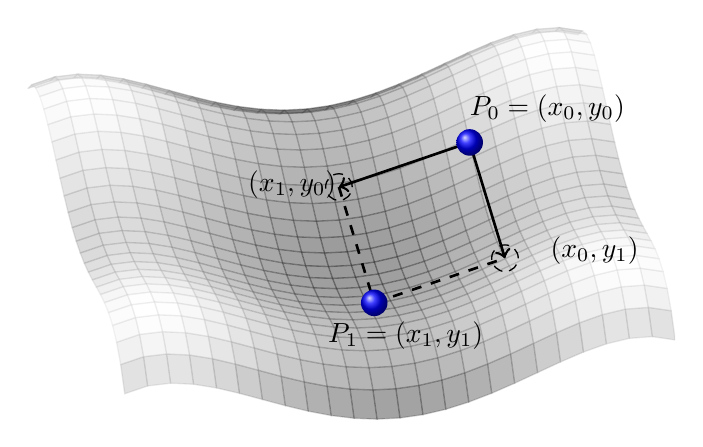
\begin{tikzpicture}[
      scale = 1.2
    ]
    \begin{axis}[
        view={-10}{60},
        zmin=-2,
        zmax=5,
        colormap/blackwhite,
        hide axis,
        xlabel=$x$,
        ylabel=$y$,
        z buffer=sort
      ]


      \addplot3 [
          surf,
          shader=faceted,
          opacity=0.2,
          fill opacity=0.4,
          samples=25,
          domain=-2:2,
          y domain=-2:2,
        ] {1.5*x^2 + 1.2*y^2 - 0.25*x^4 - 0.3*y^4};
      
      \addplot3 [
        draw=none, 
        mark=ball, 
        mark size=4, 
        z
      ] table[row sep=crcr] {%
          1     0.8     1.895\\
          0.05  -0.655  0.463 \\
        };
      
      \addplot3 [
        draw = none, 
        mark = o, 
        mark size=4,
        mark options = {
          densely dashed
        },
        z
      ] table[row sep=crcr] {%
          0.05  0.8   0.649 \\
          1     -0.655   1.710 \\
        };
      
      \addplot3 [
        <-, 
        thick, 
        black,
        z
      ] coordinates {
        (1,0.8,1.895) 
        (0.05,0.8, 0.649)
      };
      
      \addplot3 [
        -, 
        thick, 
        black,
        dashed,
        z
      ] coordinates {
        (0.05,0.8, 0.649)
        (0.05,-0.655, 0.463)
      };
      
      \addplot3 [
        ->, 
        thick, 
        black,
        z
      ] coordinates {
        (1,0.8,1.895) 
        (1,-0.655, 1.710)
      };
      
      \addplot3 [
        -, 
        thick, 
        black,
        dashed,
        z
      ] coordinates {
        (1,-0.655, 1.710)
        (0.05,-0.655, 0.463)
      };

      % \node[font=\bfseries, above] at (axis cs: 1.2, 0.8, 1.895) {$P_0 = (x_0, y_0)$};
      % \node[font=\bfseries, below] at (axis cs: 0.05, -0.655, 0.463) {$P_1 = (x_1, y_1)$};
    \end{axis}

    % \draw[step=1cm,gray,very thin] (0,0) grid (12,8);
    
    \node[font=\bfseries] at (5.5,4.1) {$P_0 = (x_0, y_0)$};
    \node[font=\bfseries] at (4,1.7) {$P_1 = (x_1, y_1)$};
    
    \node[font=\bfseries] at (6,2.6) {$(x_0, y_1)$};
    \node[font=\bfseries] at (2.8,3.3) {$(x_1, y_0)$};

  \end{tikzpicture}
\end{center}


  \end{center}
  \caption{Representação geométrica de uma etapa do método de convergência CBPD.}
  \label{fig:cbpd_geom_interp}
\end{figure}

O procedimento é repetido até atingir o critério de convergência (\ref{eq:convergence-criteria}) ou até atingir um valor máximo arbitrário de iterações.


\subsection{Avaliando Eficiência do Algoritmo}

\subsubsection{Variando uma Coordenada}

A primeira estratégia que será utilizada é, para cada ponto estacionário, como que o algoritmo se comporta quando apenas uma coordenada se distancia da conformação ideal. Nessa abordagem todas as coordendas ficam em seu valor ótimo com exceção da coordenda que está variando. Dessa maneira estaremos trabalhando com um problema em apenas uma dimensão.

Para cada ponto estacionário da reação será analisado uma coordenada relevante de cada vez, variando ela em \textit{-25\%, -20\%, -15\%, 10\%, -5\%, 0\%, 5\%, 10\%, 15\%, 20\%, 25\%} do seu valor otimizado.

Exemplificando para o caso \ce{F + H2O} haverão 11 cenários de tentativa de convergência para a primeira coordenada (Ligação \ce{H + O}) como apresentados na tabela \ref{tab:conv_one_var}. O mesmo processo será feito para todas as demais coordenadas relevantes.

\begin{table}[h]
  \centering
    \caption{Cenários de convergência do método de variação de uma coordenada para a coordenada \ce{H-O} do ponto estacionário \ce{F + H2O}}
    \label{tab:conv_one_var}
    \begin{adjustbox}{width=0.6\textwidth}
    \begin{tabular}{@{}ccccccc@{}}
      \toprule
      \multirow{2}{*}{Caso} &  \ce{H - O} & \ce{O - H$'$} & \ce{H$'$-F}  & \ce{HOH$'$}     & \ce{OH$'$F}     & \ce{HOH$'$F}  \\
          & ($x_1$) & ($x_2$) & ($x_3$) & ($x_4$) &  ($x_5$)  &  ($x_6$) \\ \midrule
      1   & 0.7207 \AA & 0.9609 \AA & 20 \AA & \ang{104.1477} & \ang{300} & \ang{300} \\ \midrule
      2   & 0.7687 \AA & 0.9609 \AA & 20 \AA & \ang{104.1477} & \ang{300} & \ang{300} \\ \midrule
      3   & 0.8168 \AA & 0.9609 \AA & 20 \AA & \ang{104.1477} & \ang{300} & \ang{300} \\ \midrule
      4   & 0.8648 \AA & 0.9609 \AA & 20 \AA & \ang{104.1477} & \ang{300} & \ang{300} \\ \midrule
      5   & 0.9128 \AA & 0.9609 \AA & 20 \AA & \ang{104.1477} & \ang{300} & \ang{300} \\ \midrule
      6   & 0.9609 \AA & 0.9609 \AA & 20 \AA & \ang{104.1477} & \ang{300} & \ang{300} \\ \midrule
      7   & 1.0089 \AA & 0.9609 \AA & 20 \AA & \ang{104.1477} & \ang{300} & \ang{300} \\ \midrule
      8   & 1.0570 \AA & 0.9609 \AA & 20 \AA & \ang{104.1477} & \ang{300} & \ang{300} \\ \midrule
      9   & 1.1050 \AA & 0.9609 \AA & 20 \AA & \ang{104.1477} & \ang{300} & \ang{300} \\ \midrule
      10  & 1.1531 \AA & 0.9609 \AA & 20 \AA & \ang{104.1477} & \ang{300} & \ang{300} \\ \midrule
      11  & 1.2011 \AA & 0.9609 \AA & 20 \AA & \ang{104.1477} & \ang{300} & \ang{300} \\ \bottomrule
    \end{tabular}%
    \end{adjustbox}
\end{table}

\subsubsection{Cenários Aleatórios de Convergência}

A segunda métrica que será utilizada busca explorar a convergência quando múltiplas coordenadas não estão em sua configuração ótima. Para isso, para cada etapa da reação química que possui a sua configuração otimizada, serão geradas 100 configurações distorciadas, nas quais a variação máxima para as ligações serão de $\pm 0.3$ \AA{} e para ângulos serão de $\pm \ang{10}$. Os valores mínimos e máximos para cada estado estácionário podem ser verificados na tabela \ref{tab:min-max-config-values}.

\begin{table}[h]
\centering
  \caption{Valores mínimos e máximos que podem ser gerados nos cenários aleatórios de convergência para cada ponto estacionário da reação \ce{F + H2O -> FH + HO}}
  \label{tab:min-max-config-values}
\resizebox{\textwidth}{!}{%
\begin{tabular}{@{}cccccccc@{}}
\toprule
  \multirow{2}{*}{Ponto Estacionário}               &            & \ce{H - O}   & \ce{O - H$'$} & \ce{H$'$-F} & \ce{HOH$'$}     & \ce{OH$'$F}     & \ce{HOH$'$F}  \\
                                                    &            &  ($x_1$)     &  ($x_2$)      &  ($x_3$)    &  ($x_4$)        &  ($x_5$)        &  ($x_6$) \\ \midrule
  \multirow{2}{*}{\ce{F + H2O}}                     & Valor Mín. & 0.6609 \AA   & 0.6609 \AA    & 19.7 \AA    & \ang{94.1477}  & \ang{290}  & \ang{290} \\ \cmidrule(l){2-8} 
                                                    & Valor Máx. & 1.2609 \AA   & 1.2609 \AA    & 20.3 \AA    & \ang{114.1477}  & \ang{310}  & \ang{310} \\ \midrule
  \multirow{2}{*}{\ce{R - vdW (F\bond{...}H2O)}}    & Valor Mín. & 0.6641 \AA   & 0.6641 \AA    & 1.9981 \AA  & \ang{94.3416}  & \ang{57.1171}  & \ang{-97.5402} \\ \cmidrule(l){2-8} 
                                                    & Valor Máx. & 1.2641 \AA   & 1.2641 \AA    & 2.5981 \AA  & \ang{114.3416}  & \ang{77.1171}  & \ang{-77.5402} \\ \bottomrule
  \multirow{2}{*}{\ce{TS}}                          & Valor Mín. & 0.6693 \AA   & 0.7270 \AA    & 1.0536 \AA  & \ang{93.2989}  & \ang{108.2898}  & \ang{58.3691} \\ \cmidrule(l){2-8} 
                                                    & Valor Máx. & 1.2693 \AA   & 1.3250 \AA    & 1.6536 \AA  & \ang{113.2989}  & \ang{128.2898}  & \ang{78.3691} \\ \bottomrule
  \multirow{2}{*}{\ce{P - vdW (HO\bond{...}HF)}}    & Valor Mín. & 0.6728 \AA   & 1.4700 \AA    & 0.6354 \AA  & \ang{98.6504}  & \ang{163.6165}  & \ang{-10.0737} \\ \cmidrule(l){2-8} 
                                                    & Valor Máx. & 1.2728 \AA   & 2.0700 \AA    & 1.2354 \AA  & \ang{118.6504}  & \ang{183.6165}  & \ang{9.9263} \\ \bottomrule
  \multirow{2}{*}{\ce{HO + HF}}                     & Valor Mín. & 0.6728 \AA   & 19.7 \AA      & 0.6223 \AA  & \ang{290}  & \ang{290}  & \ang{290} \\ \cmidrule(l){2-8} 
                                                    & Valor Máx. & 1.2728 \AA   & 20.3 \AA      & 1.2223 \AA  & \ang{310}  & \ang{310}  & \ang{310} \\ \bottomrule
\end{tabular}%
}
\end{table}

% Metodologia 
%   - Materias e Metodos
%   - Etapas da Pesquisa 
\clearpage

\section{Resultados}
\label{sec:results}

Os resultados obtidos levam em consideração a quantidade de casos que houveram convergência, e dentre esses casos, a quantidade de iterações necessárias. As informações são apresentadas de forma comparativa com o método Newton nos mesmos cenários de convergência. Todos os testes de convergência possuem um limite de 50 iterações, ao ultrapassá-lo é assumido que o algoritmo não convergiu. 

\subsection{Variando Uma Variável}
\label{sec:res-one-var}

Para os cenários onde uma variável de cada vez era afastado de seu estado otimizado, foi feita uma análise da taxa de sucesso de convergência por ponto estacionário como apresentado no gráfico \ref{fig:result-one-var-conv-tax}. Para os casos de sucesso de convergência, um gráfico de dispersão foi montado apresentando o percentual da quantidade de casos de convergência por número de iterações necessárias conforme apresentado no gráfico \ref{fig:result-one-var-conv-metric}.

\begin{figure}[h]
  \begin{subfigure}{.5\textwidth}
    \begin{center}
      \begin{center}
  
  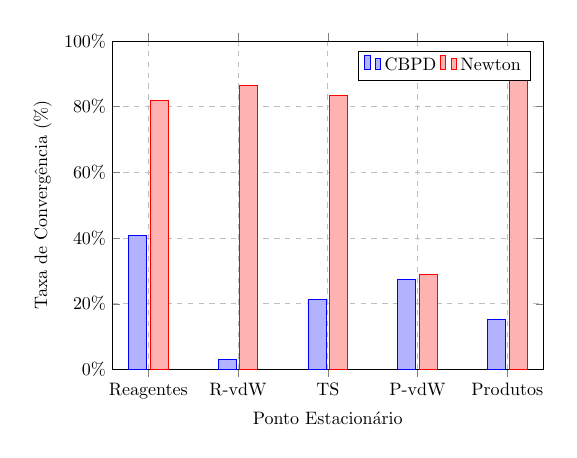
\begin{tikzpicture}[scale = 0.65]
    \begin{axis}[
      width=10cm,
      height=8cm,
      xlabel={Ponto Estacionário},
      ylabel={Taxa de Convergência (\%)},
      xtick=data,
      xticklabels={Reagentes, R-vdW, TS, P-vdW, Produtos},
      legend style={at={(0.5,-0.2)}, anchor=north, legend columns=-1},
      ymin=0,
      ymax=100,
      grid=major,
      grid style=dashed,
      ymajorgrids=true,
      ybar,
      ytick={0,20,...,100},
      yticklabel={\pgfmathprintnumber{\tick}\%},
      legend pos=north east
    ]

      \addplot[color=blue, fill=blue!30] coordinates {
        (1, 40.91)
        (2, 3.03)
        (3, 21.21)
        (4, 27.27)
        (5, 15.15)
      };

      \addplot[color=red, fill=red!30] coordinates {
        (1, 81.82)
        (2, 86.36)
        (3, 83.33)
        (4, 28.79)
        (5, 93.94)
      };

      \legend{CBPD, Newton}

    \end{axis}
  \end{tikzpicture}

\end{center}

    \end{center}
    \caption{Taxa de sucesso de convergência para os métodos iterativos CBPD e Newton para cada ponto estacionário da reação \ce{F + H2O -> FH + HO} nos casos de variação de uma variável.}
    \label{fig:result-one-var-conv-tax}
  \end{subfigure}\hspace{5mm}%
  \begin{subfigure}{.5\textwidth}
    \begin{center}
      \begin{center}
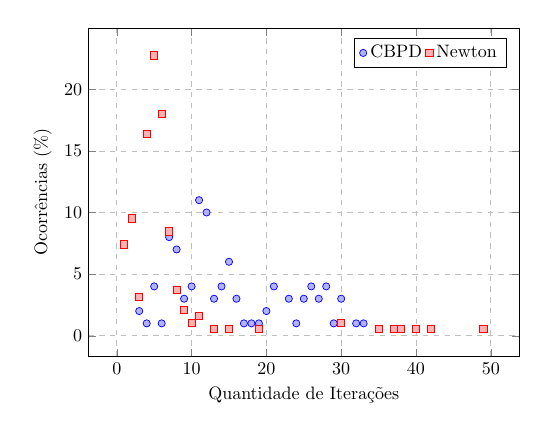
\begin{tikzpicture}[scale = 0.65]
  \begin{axis}[
    width=10cm,
    height=8cm,
    xlabel={Quantidade de Iterações},
    ylabel={Ocorrências (\%)},
    legend style={at={(0.5,-0.2)}, anchor=north, legend columns=-1},
    grid=major,
    grid style=dashed,
    legend pos=north east
  ]

    % First set of data
    \addplot[
      only marks,
      mark=*,
      color=blue,
      fill=blue!30,
    ] coordinates {
        (12, 10.00)
        (11, 11.00)
        (5, 4.00)
        (13, 3.00)
        (14, 4.00)
        (15, 6.00)
        (9, 3.00)
        (7, 8.00)
        (23, 3.00)
        (16, 3.00)
        (8, 7.00)
        (30, 3.00)
        (32, 1.00)
        (19, 1.00)
        (33, 1.00)
        (21, 4.00)
        (20, 2.00)
        (25, 3.00)
        (26, 4.00)
        (28, 4.00)
        (27, 3.00)
        (29, 1.00)
        (10, 4.00)
        (18, 1.00)
        (17, 1.00)
        (24, 1.00)
        (6, 1.00)
        (4, 1.00)
        (3, 2.00)
      };

    % Second set of data
    \addplot[
      only marks,
      mark=square*,
      color=red,
      fill=red!30,
    ] coordinates {
        (6, 17.99)
        (5, 22.75)
        (4, 16.40)
        (2, 9.52)
        (7, 8.47)
        (3, 3.17)
        (9, 2.12)
        (8, 3.70)
        (10, 1.06)
        (11, 1.59)
        (35, 0.53)
        (38, 0.53)
        (40, 0.53)
        (30, 1.06)
        (13, 0.53)
        (1, 7.41)
        (15, 0.53)
        (49, 0.53)
        (42, 0.53)
        (37, 0.53)
        (19, 0.53)
    };
    \legend{CBPD, Newton}

  \end{axis}
\end{tikzpicture}
\end{center}

    \end{center}
    \caption{Percentual da quantidade de iterações necessárias para convergir para os métodos iterativos CBPD e Newton para a reação \ce{F + H2O -> FH + HO} nos casos de variação de uma variável.}
    \label{fig:result-one-var-conv-metric}
  \end{subfigure}
  \caption{Resultados dos casos de variação de uma variável.}
\end{figure}

\subsection{Cenários Aleatórios de Convergência}

Para os cenários de convergência nos quais todas as variáveis são aleatorizadas, foi feita uma análise similar à descrita na seção \ref{sec:res-one-var}. Uma análise da taxa de convergência por ponto estacionário é apresentada no gráfico \ref{fig:result-mult-var-conv-tax}, enquanto para os casos de sucesso convergência, um gráfico de dispersão foi montado apresentando o percetual da quantidade de casos de convergência por número de interações conforme apresentado no gráfico \ref{fig:result-mult-var-conv-metric}.

\begin{figure}[h]
  \begin{subfigure}{.5\textwidth}
    \begin{center}
    \begin{center}
  
  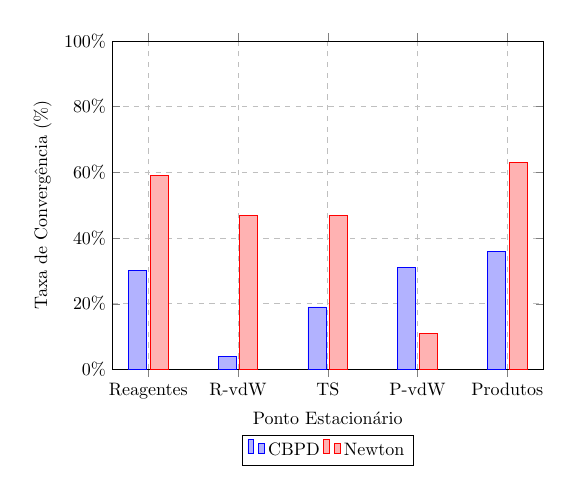
\begin{tikzpicture}[scale = 0.65]
    \begin{axis}[
      width=10cm,
      height=8cm,
      xlabel={Ponto Estacionário},
      ylabel={Taxa de Convergência (\%)},
      xtick=data,
      xticklabels={Reagentes, R-vdW, TS, P-vdW, Produtos},
      legend style={at={(0.5,-0.2)}, anchor=north, legend columns=-1},
      ymin=0,
      ymax=100,
      grid=major,
      grid style=dashed,
      ymajorgrids=true,
      ybar,
      ytick={0,20,...,100},
      yticklabel={\pgfmathprintnumber{\tick}\%}
    ]

      \addplot[color=blue, fill=blue!30] coordinates {
        (1, 30.00)
        (2, 4.00)
        (3, 19.00)
        (4, 31.00)
        (5, 36.00)
      };

      \addplot[color=red, fill=red!30] coordinates {
        (1, 59.00)
        (2, 47.00)
        (3, 47.00)
        (4, 11.00)
        (5, 63.00)
      };

      \legend{CBPD, Newton}

    \end{axis}
  \end{tikzpicture}

\end{center}

    \end{center}
    \caption{Taxa de sucesso de convergência para os métodos iterativos CBPD e Newton para cada ponto estacionário da reação \ce{F + H2O -> FH + HO} nos cenários aleatórios de convergência.}
    \label{fig:result-mult-var-conv-tax}
  \end{subfigure}\hspace{5mm}%
  \begin{subfigure}{.5\textwidth}
    \begin{center}
    \begin{center}
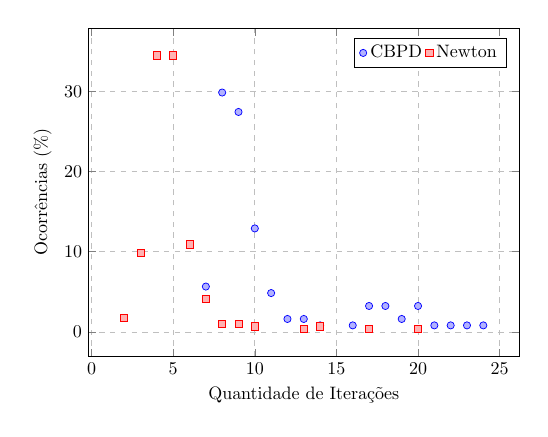
\begin{tikzpicture}[scale = 0.65]
  \begin{axis}[
    width=10cm,
    height=8cm,
    xlabel={Quantidade de Iterações},
    ylabel={Ocorrências (\%)},
    legend style={at={(0.5,-0.2)}, anchor=north, legend columns=-1},
    grid=major,
    grid style=dashed,
    legend pos=north east
  ]

    % First set of data
    \addplot[
      only marks,
      mark=*,
      color=blue,
      fill=blue!30,
    ] coordinates {
        (9, 27.42)
        (10, 12.90)
        (8, 29.84)
        (7, 5.65)
        (11, 4.84)
        (13, 1.61)
        (12, 1.61)
        (18, 3.23)
        (20, 3.23)
        (23, 0.81)
        (24, 0.81)
        (22, 0.81)
        (17, 3.23)
        (19, 1.61)
        (14, 0.81)
        (21, 0.81)
        (16, 0.81)
      };

    % Second set of data
    \addplot[
      only marks,
      mark=square*,
      color=red,
      fill=red!30,
    ] coordinates {
        (4, 34.47)
        (5, 34.47)
        (3, 9.90)
        (2, 1.71)
        (6, 10.92)
        (8, 1.02)
        (7, 4.10)
        (10, 0.68)
        (17, 0.34)
        (13, 0.34)
        (9, 1.02)
        (14, 0.68)
        (20, 0.34)
    };
    \legend{CBPD, Newton}

  \end{axis}
\end{tikzpicture}
\end{center}

    \end{center}
    \caption{Percentual da quantidade de iterações necessárias para convergir para os métodos iterativos CBPD e Newton para a reação \ce{F + H2O -> FH + HO} nos cenários aleatórios de convergência.}
    \label{fig:result-mult-var-conv-metric}
  \end{subfigure}
  \caption{Resultados dos cenários aleatórios de convergência.}
\end{figure}

Avaliando as taxas de convergências dos métodos CBPD e Newton é notório que o método de Newton apresenta melhores resultados de convergência na maioria dos pontos estacionários da reação com exceção do $P-vdW$. Em termos de quantidades de iterações necessárias para convergência, o Método de Newton apresenta uma maior consistência, sendo necessário em torno de 5 a 7 iterações. Já no Método CBPD a quantidade de iterações necessárias possui um pico entre 11 e 12 iterações.

\clearpage

\section{Conclusões}
\label{sec:conclusions}

A presente pesquisa permitiu explorar um novo método iterativo aplicado em um cenário real, de maneira comparativa com o método de Newton e permitindo evidenciar resultados positivos e negativos em diferentes cenários de convergência, avaliando seu desempenho baseando-se principalmente na quantidade de iterações necessárias para convergir.

Apesar do Método CBPD possuir uma quantidade de iterações necessárias para convergir próximas do dobro de iterações quanto comparado com o Método de Newton, é válido levar em consideração o custo computacional envolvido no processamento de ambos os algoritmos. No método CBPD, para cada iteração possui uma complexidade $O(n)$ para ser calculada, considerando $n$ a quantidade de parâmetros da função a ser otimizada. Já no Método de Newton, possui uma complexidade $O(n^3)$ decorrente da necessidade de inversão da matriz hessiana $n \times n$.

É válido seguir os estudos nessa pesquisa para analisar os critérios formais de convergência para o método caso existam, que podem estar relacionados com casos em que a matriz hessiana é diagonalizável e o valor dos elementos de sua matriz diagonal seja suficientemente próximos dos autovetores da matriz. Esse entendimento permite predizer com mais assertividade os cenários em que é vantajoso a utilização do método.

Ademais é relevante analisar especificamente o caso de convergência para o ponto estacionário P-vdW, em que o método CBPD apresentou uma taxa de convergência consideravelmente superior ao do método de Newton, resultado esse não esperado, visto que o método de Newton tende a ser mais estável nos casos de convergência.

\clearpage

%%%%%%%%%%%%%%%%%%%%%%%%%%%%%%%%%%%%%%%%%% Final %%%%%%%%%%%%%%%%%%%%%%%%%%%%%%%%%%%%%%%%%%
%\section{Referências}
\newpage
%\bibliography{ref} % Entries are in the refs.bib file
%\printbibliography
%\end{boldmath}
\bibliography{ref}{}
\bibliographystyle{plain}
\end{document}
